\documentclass[border=3pt,tikz]{standalone}
\usepackage{amsmath}
\usetikzlibrary {arrows.meta}
\usetikzlibrary {calc}
\usetikzlibrary {math}

\begin{document}
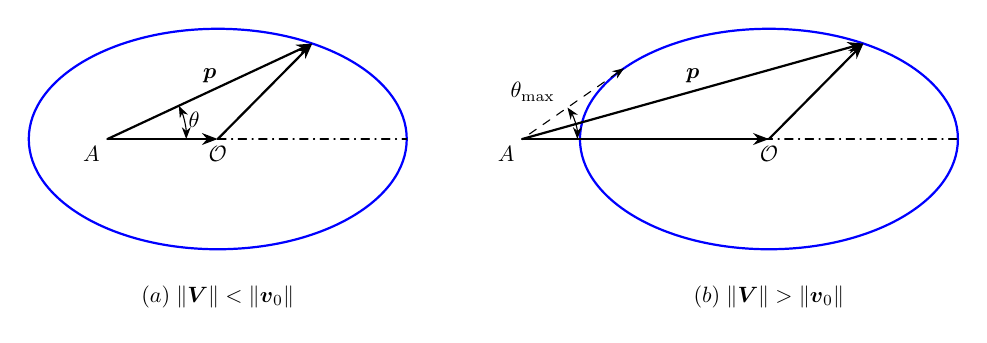
\begin{tikzpicture}[line cap=round, scale = 2]

    \begin{scope}[shift={(0,0)}]
        \tikzmath{
            \a = 1.2;
            \b = 0.7;	
            \th1 = 60;
            \Ax = -0.7;
            \Rth = 0.5;
        };
        \coordinate (P1) at ({\a*cos(\th1)}, {\b*sin(\th1)});
        \coordinate (O) at (0, 0);
        \draw[fill=none, blue, thick](0,0) ellipse ({\a} and {\b});
        \draw[dashdotted] (0, 0) -- (\a, 0);
        \draw[thick,  -{Stealth[length=2mm]}] (0, 0) -- (P1);

        \node [below, scale=0.8] at (O) {$\mathcal{O}$};
        
        \draw[thick,  -{Stealth[length=2mm]}] (-0.7, 0)  -- (0, 0);
        \node[below left, scale=0.8] at (\Ax, 0) {$A$};
        
        \draw [{Stealth[length=1.5mm]}-{Stealth[length=1.5mm]}] ({\Ax + \Rth},0.0) arc (0:25:\Rth);
        \node[scale=0.8] at (-0.15 , 0.12) {$\theta$};
        
        
        \draw[thick,  -{Stealth[length=2mm]}] (-0.7, 0)  -- node[above, scale = 0.8] {$\boldsymbol{p}$}(P1);
        \node[scale=0.8] at(0.0, -1.0) {$(a)\; \|\boldsymbol{V}\|<\|\boldsymbol{v}_0\|$};
        
    \end{scope}
    
    \begin{scope}[shift={(3.5,0)}]
		\tikzmath{
            \a = 1.2;
            \b = 0.7;	
            \th1 = 60;
            \th2 = 140;
            \tt = {-\b/\a*cos(\th2)/sin(\th2)};  
            \thmax = atan2(\b*sin(\th2), \a*cos(\th2) -\a/cos(\th2) );
            \Rth = 0.35;
            \Ax = \a/cos(\th2);
        };
        \coordinate (O) at (0, 0);
        \coordinate (P1) at ({\a*cos(\th1)}, {\b*sin(\th1)});
        \coordinate (P2) at ({\a/cos(\th2)}, {0});
        \coordinate (P3) at ({\a*cos(\th2)}, {\b*sin(\th2)});
        \draw[fill=none, blue, thick](0, 0) ellipse ({\a} and {\b});;
        \draw[dashdotted] ({-\a}, {0}) -- (\a, 0);
        
        \draw[thick,  -{Stealth[length=2mm]}] (P2)  -- (O);
        \node[below left, scale=0.8] at (P2) {$A$};
        \draw[thick,  -{Stealth[length=2mm]}] (O) -- (P1);
        \draw[dashed, {Stealth[length=1.5mm]}-] (P3) -- (P2);

        \node [below, scale=0.8] at (O) {$\mathcal{O}$};
                
        
        \draw [{Stealth[length=1.5mm]}-{Stealth[length=1.5mm]}] ({\Ax+\Rth},{0.0}) arc (0:{\thmax}:{\Rth});
        \node[scale=0.8] at (-1.5, 0.3) {$\theta_\textrm{max}$}; 
        
        \draw[thick,  -{Stealth[length=2mm]}] (P2) -- node[above, scale=0.8] {$\boldsymbol{p}$} (P1);
                
        \node[scale=0.8] at(0, -1.0) {$(b)\; \|\boldsymbol{V}\|>\|\boldsymbol{v}_0\|$};
        
    \end{scope}
    \end{tikzpicture}
\end{document}